\begin{frame}
  \frametitle{Modele Markov Complet}
  \begin{block}{Modele Markov Complet}
    Un lanț Markov se numește \alert{complet} dacă din orice stare se poate ajunge în oricare altă stare direct.\\
    Matricea de tranziție nu are nicio valoare nulă.
  \end{block}
  \vspace*{1em}
  \begin{center}
    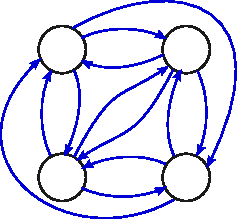
\includegraphics[width=0.4\textwidth]{graphics/other-hmm/full.pdf}
  \end{center}
\end{frame}


\begin{frame}
  \frametitle{Modele Markov Ergodice}
  \begin{block}{Modele Markov Ergodice}
    Un lanț Markov se numește \alert{ergodic} dacă din orice stare se poate ajunge în oricare altă stare (nu neaparat într-o singură mutare).\\
    Lanțurile Markov ergodice se mai numesc și \emph{ireductibile}.
  \end{block}
  \vspace*{1em}
  \begin{center}
    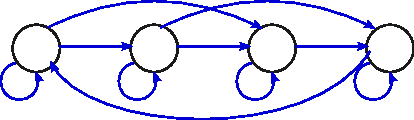
\includegraphics[width=0.8\textwidth]{graphics/other-hmm/ergodic.pdf}
  \end{center}
\end{frame}

\begin{frame}
  \frametitle{Modelul Bakis}
  \begin{block}{Modele Markov Bakis (stânga $\longrightarrow$ dreapta)}
    Un model \alert{Bakis} este unul în care nu este permisă tranziția
    dintr-o stare către o altă stare cu un indice mai mic.
  \end{block}
  \vspace*{1em}
  \begin{center}
    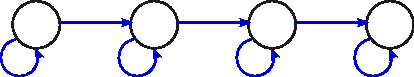
\includegraphics[width=0.8\textwidth]{graphics/other-hmm/left-to-right.pdf}
  \end{center}
\end{frame}

\begin{frame}
  \frametitle{Alte tipuri de MMA}
  \begin{itemize}
  \item modele Markov cu memorie mixă \citep{Saul:1999:MMM:326214.325611}
    \begin{itemize}
    \item scalează mai bine cu secvențe de lungime mare
    \item utile în: modelarea vizitării paginilor web
    \end{itemize}
    \vspace*{.5em}
  \item modele Markov ascunse de durată variabilă \citep{rabiner1989tutorial}
    \begin{itemize}
    \item utile în: recunoașterea cuvintelor scrise cursiv de mână \citep{chen1995variable}
    \end{itemize}
    \vspace*{.5em}
  \item modele Markov ascunse factoriale \citep{Ghahramani97factorialhidden}
    \begin{itemize}
    \item mai multe variabile de stare
    \item putere de modelare mai mare
    \item algoritmi exacți intractabili
    \end{itemize}
    \vspace*{.5em}
  \item modele Markov ascunse ierarhice \citep{fine1998hierarchical}
    \begin{itemize}
    \item utile în: recunoașterea scrisului de mână cursiv
    \end{itemize}
  \end{itemize}
\end{frame}